%----------------------------------------------------------------------------------------
%	Inställningar och dokumentkonfiguration
%----------------------------------------------------------------------------------------

\documentclass[paper=a4, fontsize=11pt]{report} % A4-sida och 11 punkters fontstorlek

\usepackage[T1]{fontenc} % 8-bitarskodning som har 256 glyfer
\usepackage[english]{babel} % Svenskt språk(ändrat till engelska)
\usepackage[utf8]{inputenc} % För svenska tecken
\usepackage{dtklogos} % Logos
\usepackage{wallpaper} % Bakgrundsbild
\usepackage{fancyhdr} % Specialsidhuvud och sidfot
\usepackage{enumerate} 
\usepackage{hyperref}
\usepackage{textcomp}
\usepackage{xifthen}% provides \isempty test
\pagestyle{fancyplain} % Använd sidhuvud och sidfot på alla sidor
\fancyhead[L]{Laboration 1 -- 1DV020 -- VT15 -- Server administraion I} % Titel till vänster i sidhuvud
\fancyhead[C]{} % Tomt i mitten
\fancyhead[R]{} % Tomt till höger
\fancyfoot[L]{{\color{gray}\textcopyright \ 2015 Jacob Lindehoff, Kristoffer Schill}} % Tomt till vänster
\fancyfoot[C]{}  % Tomt i mitten
\fancyfoot[R]{\thepage} % Sidnumrering till höger i sidfoten
\renewcommand\thesection{\arabic{section}} % Section beter sig som i dokumentklassen article

\newcommand{\win}[1]{Microsoft Windows Server\ifthenelse{\isempty{#1}}{}{ #1}}
\newcommand{\gui}[0]{``Server with a GUI''}
\newcommand{\core}[0]{Windows Server Core}
%----------------------------------------------------------------------------------------
%	TITLE SECTION
%----------------------------------------------------------------------------------------
\newcommand\BackgroundPic{
    \put(-50,-50){
    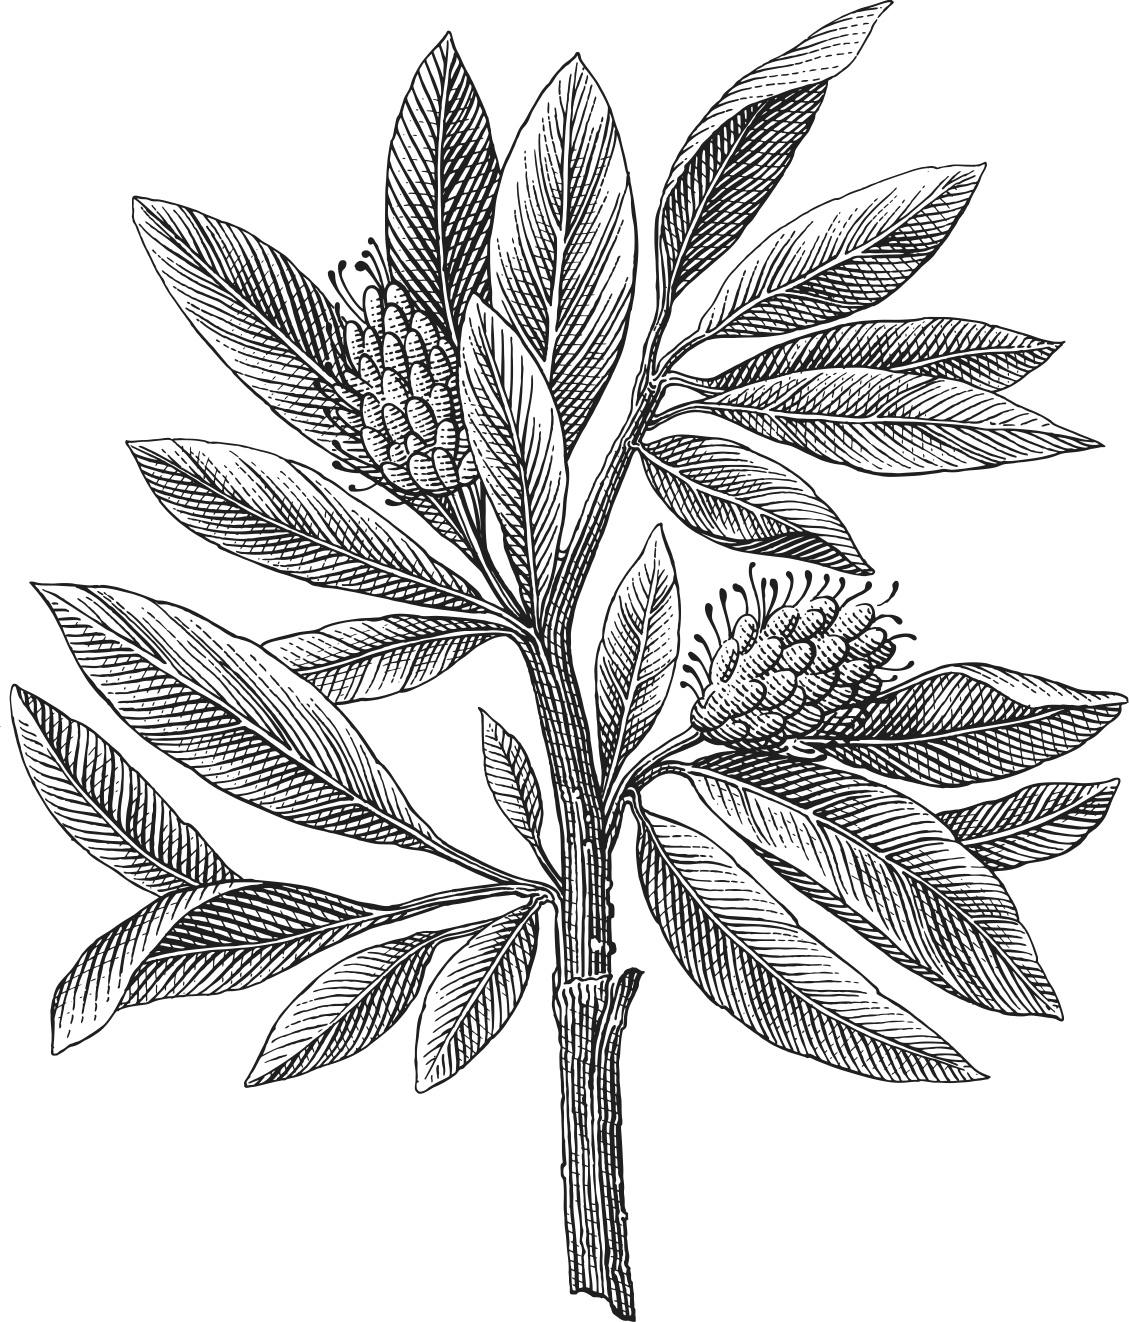
\includegraphics[keepaspectratio,scale=0.65]{lnu_etch.png} % Bakgrundsbild
    }
}
\newcommand\BackgroundPicLogo{
    \put(15,700){
    
\includegraphics[keepaspectratio,scale=0.10]{logo.png} % Logga i vänstra hörnet
    }
}

\newcommand{\horrule}[1]{\rule{\linewidth}{#1}} % Skapa hortisontell linje

\title{	\vspace{-10cm}
    \normalfont \normalsize
    \textsc{Linnéuniversitetet} \\ [25pt] % Universitetes namn
    \horrule{0.5pt} \\[0.4cm] % Tunn linje högst upp
    \huge Laboration 1\\ % Arbetes titel
	\large \textcolor{gray}{1DV416 -- Windowsadministraion I}
    \horrule{0.5pt} \\[0.4cm] % Tunn linje längst ner
}

% \author{Jacob Lindehoff} % Författarnas namn

\date{\normalsize\today} % Dagens datum

\begin{document}
\AddToShipoutPicture*{\BackgroundPic} % Lägger in backgrundsbild på första sidan
\AddToShipoutPicture*{\BackgroundPicLogo}
\maketitle % Skriv ut titeln
\noindent % Tabba inte in på första meningen

%------------------------------------------------
%	Introduction
%------------------------------------------------
\section{Introduction}

You are an IT-technican on a small newly founded company and the board have given you the task to install the company's first servers and clients. There are some requirements on the system that you should find in the Chapter~\ref{tasks}

It is importaint that you have read the lab thoroughly before you start with the laboration. You must follow the instructions on the course page or under chapter ~\ref{enviroment}.

All machines that are created are saved under your own folder in: ... 
Alla maskiner som skapas ska sparas på L: under din egna mapp i 1DV416: \textbf{L:\textbackslash VirtualLabs\textbackslash Courses\textbackslash 1DV416\textbackslash users\textbackslash 2013\textbackslash [Ditt Användarnamn]\textbackslash }

%------------------------------------------------
%	Deadline
%------------------------------------------------
\section{Deadline}

There are two laboratory sessions connected to this module, at these sessions you are given the opportunity to get help if swo needed. To be able to finish the modules you are likely needed to spend more time on your own.

\paragraph{Accounting} You will show your work and demonstrate your progress at any of these labsession, prepare a small document with an overview of your configuration/setup if needed for overview.

\pagebreak
%------------------------------------------------
%	Uppgift
%------------------------------------------------
\section{Assignment}
\begin{figure}[h]
\centering
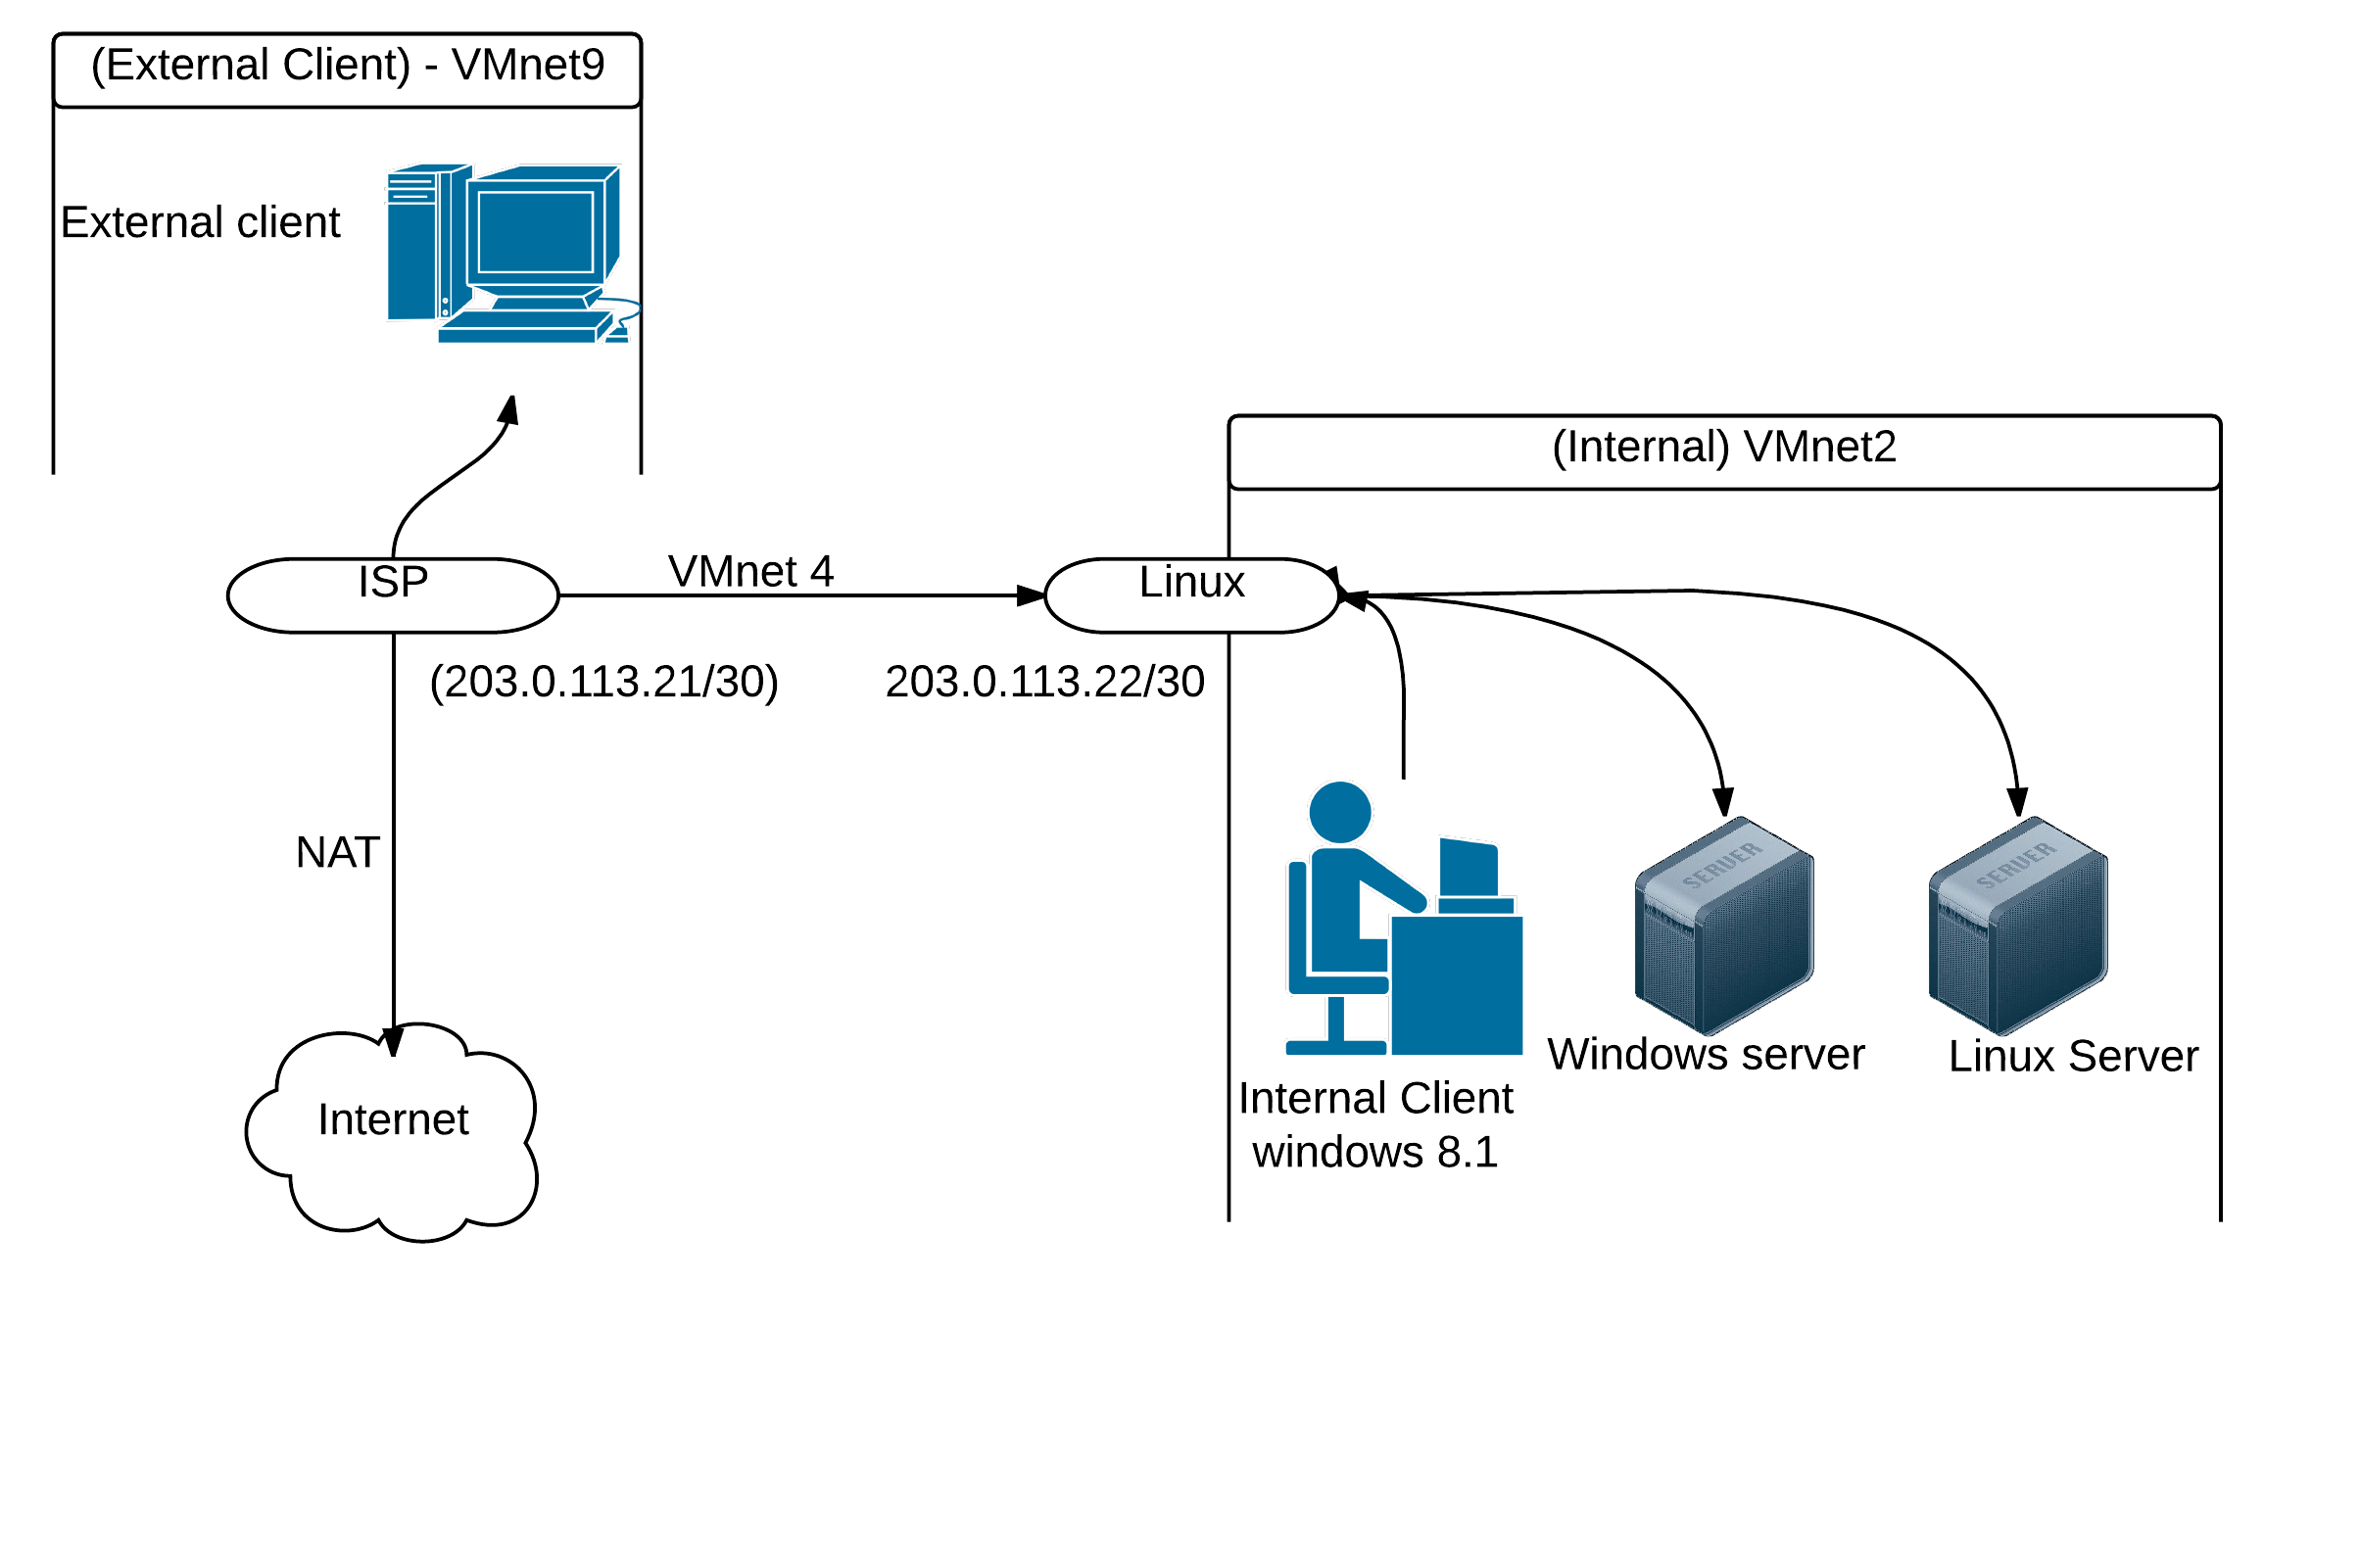
\includegraphics[width=1\linewidth]{./network}
\caption[Figur över nätverket i labb 1]{The network as it should be setup in Labb 1.}
\label{fig:network}
\end{figure}

You have been given the the task to setup a newly founded company's network. In \figurename \ref{fig:network} you should see how the network should look when you are done with lab 1.

Det är ett mycket enkelt nätverk ni ska sätta upp med en filserver och två klienter. För att komma ut på Internet så måste ni även sätta upp en server som agerar router mellan LANet och Internet.

The topology contains one Linux server, one Windows server, one Linux router and one client. Using the linux router as a gateway all the devices should be able to reach the internet.

\section{Krav}
\label{tasks}
Utöver nätverksskissen har ni fått en del krav som företaget har satta upp:

\begin{itemize}
    \item Alla maskiner ska:
    \begin{itemize}
        \item should be configured as the networksketch in \figurename \ref{fig:network}
        \item köra statisk IP-adressering, nätadresser får ni själva välja men motivera ert val i labbrapporten
        \item have static ip-addressing, the addresses is up to you to decide but you should be able to motivate your choice. 
		\item should have internet access using the linux router.
        \item have proper firewall rules. This includes both the linux and windows machines.
    \end{itemize}
    \item Should be able to ping all the devices on the LAN.
    \item Have a proper naming convention.
	\item Specifika maskinkrav:
    \begin{itemize}
        \item \textbf{ISP Gateway}
        \begin{itemize}
            
			\item This is the only machine that you will not install yourself, it is a predefined machine that you will make a linked clone of.
            \item The template is located at \textbf{\textbackslash\textbackslash: VirtualLabs\textbackslash Files\textbackslash Templates\textbackslash ISP Gateway Template\textbackslash }
        \end{itemize}

        \item \textbf{Linuxrouter}
        \begin{itemize}
			\item should have two network cards, one for the WAN and one for the local LAN.
            \item The WANet should be configured according to the network sketch in \figurename \ref{fig:network}, \textit{Observe! To be able to lookups it needs to use the ISP Gateways DNS server.}
			
        \end{itemize}
    \end{itemize}
\end{itemize}

\section{Workenviroment}
\label{enviroment}

You will be using VMware Workstation to be able to accomplish this lab. You will only use templates for the ISP Gateway in this lab. The rest is up to you to construct from isofiles.
 
To be able to start this laboration you need to have signed up for MSNDAA and a labbgroup. When you have done this it takes up to a workday before you are put into the system.

\paragraph{ISO} Till din hjälp så finns \win{2012 R2} och Windows 8.1 ISOs på 

L:\textbackslash VirtualLabs\textbackslash Files\textbackslash CD\textbackslash Microsoft\textbackslash 
\begin{itemize}
\item 9600.16384.WINBLUE\_RTM.130821-1623\_X64FRE\_SERVER\_EVAL\_EN-US-IRM\_SSS\_X64FREE\_EN-US\_DV5.ISO
\item 9600.16384.WINBLUE\_RTM.130821-1623\_X64FRE\_ENTERPRISE\_EVAL\_EN-US-IRM\_CENA\_X64FREE\_EN-US\_DV5.ISO
\end{itemize}
Windows 7 ISOn hittar du här: \textbf{L:\textbackslash VirtualLabs\textbackslash Files\textbackslash MSDNAA\textbackslash Operating Systems\textbackslash en\_windows\_7\_enterprise\_with\_sp1\_x64\_dvd\_620201.iso
}\end{document}
